% Requires texlive-latex-recommended and texlive-fonts-recommended packages (Debian, Ubuntu).
%%%%%%%%%%%%%%%%%%%%%%%%%%%%%%%%%%%%%%%%%% NEW MAXIMUM LINE LENGTH (120 char) %%%%%%%%%%%%%%%%%%%%%%%%%%%%%%%%%%%%%%%%%%
\documentclass[a4paper,oneside,openany,12pt]{memoir}
\usepackage[T1]{fontenc} % To get different font encoding, thus allow \guillemotright.
% Undo bad "side effects" of T1 font encoding (ugly font && chapters in small caps).
% Note that it's now not shown in small caps simply because the selected font does not support it.
\usepackage{lmodern}
\usepackage{graphicx} % For images
\graphicspath{{../gfx/}}
%\usepackage[english]{babel} % For correct word hyphenating.
\usepackage{color}    % For colored links and boxes.
\usepackage[dvipsnames]{xcolor}
\definecolor{LOVDdark}{HTML}{224488}
\definecolor{LOVDlight}{HTML}{F0F3FF}
\usepackage{float}    % For custom floats (the info boxes).
\usepackage{wrapfig}  % For floating boxes meant for small notes.
% When loaded before float, doesn't work.
% For figures, maybe not do an frame but a box without border and with background color?
\usepackage[format=hang,font=footnotesize,labelfont=bf,skip=5pt]{caption} % To format captions.
\usepackage{hyperref} % For URLs.
\usepackage{tikz}
\usepackage{xr}

% Include all of this in a separate file!
\newcommand{\HRule}{\rule{\linewidth}{1mm}} % Doet height (zie style) hetzelfde?
\newcommand{\institute}[1]{\gdef\inst{#1}}  % Beamer supplies \institute. We want that, too.
\newcommand{\inst}{}                        % Beamer supplies \institute. We want that, too.
\newcommand{\funding}[1]{\gdef\fund{#1}}    % Provide funding line.
\newcommand{\fund}{}                        % Provide funding line.
\newcommand{\setcreativecommons}[1]{\gdef\creativecommons{#1}}	% Provide creative commons line.
\newcommand{\creativecommons}{}                       			 		% Provide creative commons line.
\newcommand{\setLOVDversion}[1]{\gdef\LOVDversion{#1}} % Provide the current LOVD version.
\newcommand{\LOVDversion}{}                            % Provide the current LOVD version.
\newcommand{\setpointercolor}[1]{\gdef\pointercolor{#1}}%
\newcommand{\pointercolor}{}  													%
\newcommand{\setpointerwidth}[1]{\gdef\pointerwidth{#1}}%
\newcommand{\pointerwidth}{}  													%
\newcommand{\setgrid}[1]{\gdef\drawgrid{#1}}						% Used for drawing a grid over a figure
\newcommand{\drawgrid}{} 																%
\newcommand{\setmanualversion}[1]{\gdef\manualversion{#1}} 	% Provide the current manual version.
\newcommand{\manualversion}{}                            		% Provide the current manual version.

\setlrmarginsandblock{2cm}{2cm}{*} % LEFT-RIGHT
\setulmarginsandblock{2cm}{2cm}{*} % TOP-BOTTOM
\checkandfixthelayout % Without this, nothing works. Took me ages before I found out.
\fixpdflayout % Not sure if we need this, but it was recommended someplace.



%%%%% PAGE HEADERS AND FOOTERS %%%%%
\makepagestyle{LOVD}

% Because we don't have odd or even pages, we only need to define odd pages.
\makeoddhead{LOVD}{\normalfont\leftmark}{}{\normalfont\rightmark}
\makeheadrule{LOVD}{\textwidth}{\normalrulethickness}
\makeoddfoot{LOVD}{}{\normalfont\thepage}{}
\makefootrule{LOVD}{\textwidth}{\normalrulethickness}{\footruleskip}

% Style "plain" is called from chapters. We want chapters to have a footer as well.
\makeoddfoot{plain}{}{\normalfont\thepage}{}
\makefootrule{plain}{\textwidth}{\normalrulethickness}{\footruleskip}

% Additional changes:
\makepsmarks{LOVD}{%
  \nouppercaseheads

  \createmark{chapter}{left}{shownumber}{}{.\space} % (\leftmark) number, followed by a . and a space.
  \createmark{section}{right}{nonumber}{}{.\space} % (\rightmark) no number, (useless: followed by a . and a space).
  % Change "shownumber" to "nonumber" if you don't want the chapter/section number displayed at the header.
}
% Activate your new pagestyle
\pagestyle{LOVD}



%%%%% TITLE PAGE FORMAT %%%%%
\setlength{\droptitle}{-3cm} % Moves the title (logo, title, authors etc) 3cm up.
\pretitle{
  \begin{center}
    \vskip 3cm
    
\includegraphics[width=16cm]{logo_plus.png}
    \vskip 1.5cm
%    
\includegraphics[width=3cm]{hgvs.png} \hspace{1.5cm}
%    
\includegraphics[width=3cm]{human_variome.png} \hspace{1.5cm}
%    
\includegraphics[width=3cm]{gen2phen.jpg}
    \vskip 3cm
    \HRule\par\HUGE\bfseries\sffamily} %% Need proper font!
\posttitle{\par\HRule\end{center}\vskip 2cm}
\preauthor{\flushright \vskip12em}
\postauthor{\par\inst\par\vskip 5mm}
\predate{\hfill  Last updated: }
\postdate{
  \par\clearpage \hfill 
  \vskip42em

  \noindent
  We have chosen GeneticReports as our partner to provide support and hosting for LOVD\textsuperscript{+}.
  If you're interested in getting support setting up LOVD\textsuperscript{+}
   in your institute or are looking for a provider to host LOVD\textsuperscript{+} for you,
   please see \url{http://geneticreports.org/}.
  GeneticReports is a young, innovative company that provides genetic reports that
   can provide diagnosis as well as help predict the likelihood of developing a particular
   disease before symptoms occur, using data from LOVD databases.
  \vskip1em
  \noindent
  For more information regarding the LOVD\textsuperscript{+} software, please see \url{http://LOVD.nl/plus}.

  \vskip2em
  \small \noindent \creativecommons
} 



%%%%% CHAPTER STYLE (CHAPTER HEADS) %%%%%
\makechapterstyle{LOVD}{%
  \setlength\beforechapskip{10pt} % A small distance just above the new Chapter title.
  \setlength\afterchapskip{20pt} % A small distance between the Chapter title and the text.
  \renewcommand{\chapterheadstart}{\vspace*{\beforechapskip}\hrule height 2pt \medskip} % Nice ruler above the Capter title.
  \renewcommand{\chapnamefont}{\normalfont\large\scshape} % CHAPTER
  \renewcommand{\chapnumfont}{\normalfont\huge\bfseries\scshape} % 1
  \renewcommand{\chaptitlefont}{\normalfont\huge\bfseries\scshape} % e.g. "Introduction"
  \renewcommand{\printchaptername}{} % Empty text instead of "Chapter".
                  \renewcommand{\chapternamenum}{ } % Weet niet wat dit anders doet.
                  \renewcommand{\printchapternum}{\chapnumfont \thechapter} % Weet niet wat dit anders doet.
  \renewcommand{\afterchapternum}{. } % Just a dot after the Chapter number, no new line.
  \renewcommand{\afterchaptertitle}{\par\nobreak\medskip\hrule\vskip\afterchapskip} % Nice ruler below the Capter title.
}
\chapterstyle{LOVD}



%%%%% LINK CONFIGURATION %%%%%
\definecolor{linkblue}{rgb}{0.1, 0, 1}
\hypersetup{
  colorlinks,
  citecolor=linkblue,
  filecolor=linkblue,
  linkcolor=linkblue,
  urlcolor=linkblue
}



%%%%% INFOTABLE AND WARNTABLE DEFINITIONS %%%%%
\newsavebox{\infobox}
\newlength{\infoboxlength}
\newlength{\infoboxinnerlength}
\setlength{\infoboxlength}{\textwidth}
\addtolength{\infoboxlength}{-2\fboxsep}
\addtolength{\infoboxlength}{-2\fboxrule}
\addtolength{\infoboxlength}{-1.7cm} % Manually configured value making sure the whole box doesn't exceed the line width.
\setlength{\infoboxinnerlength}{\infoboxlength}
\addtolength{\infoboxinnerlength}{-5pt} % Manually configured value making sure the text doesn't get too near the right border.

%%%%%% DEFINITIONS FOR \FBOX %%%%%%%
\setlength{\fboxsep}{2pt}%
\setlength{\fboxrule}{2pt}%

\newenvironment{infotable}
  {\begin{lrbox}{\infobox}%
    \begin{minipage}[t]{1.5cm}
      \centering
      \vspace{0pt}
      
\includegraphics[width=1cm,height=1cm]{lovd_information.png}
    \end{minipage}
   \begin{minipage}[t]{\infoboxlength}\vspace{5pt}\begin{minipage}{\infoboxinnerlength}}
  {\vspace{6pt}\end{minipage}\end{minipage}\end{lrbox}%
   \begin{center}
   \fcolorbox{black}{LOVDlight}{\usebox{\infobox}}
   \end{center}}

\newenvironment{warntable}
  {\begin{lrbox}{\infobox}%
    \begin{minipage}[t]{1.5cm}
      \centering
      \vspace{0pt}
      
\includegraphics[width=1cm,height=1cm]{lovd_warning.png}
    \end{minipage}
   \begin{minipage}[t]{\infoboxlength}\vspace{5pt}\begin{minipage}{\infoboxinnerlength}}
  {\vspace{6pt}\end{minipage}\end{minipage}\end{lrbox}%
   \begin{center}
   \fcolorbox{black}{LOVDlight}{\usebox{\infobox}}
   \end{center}}



%%%%% CONFIGURE LEFTBAR (FRAMED PACKAGE) %%%%%
% Taken and adapted from http://tex.stackexchange.com/questions/22526/regarding-the-leftbar-environment
% (thanks, xport & Martin Scharrer)
% I still don't like the space between the bar and the colorbox (can be removed by taking out the \hspace), but
% I want that space *inside* the colorbox.
\renewenvironment{leftbar}[1][\hsize]
{%
    \def\FrameCommand
    {%
        {\color{LOVDdark}\vrule width 3pt \hspace{5pt}}%
        \colorbox{LOVDlight}%
    }%
    \MakeFramed{\hsize#1\advance\hsize-\width\FrameRestore}%
}
{\endMakeFramed}



%%%%% CONFIGURE IMAGES %%%%%
\definecolor{shadecolor}{RGB}{240, 243, 255} %F0F3FF
\setgrid{\draw[help lines,xstep=.05,ystep=.05] (0,0) grid (1,1);
	\foreach \x in {0,1,...,9} { \node [anchor=north] at (\x/10,0) {0.\x}; }
	\foreach \y in {0,1,...,9} { \node [anchor=east] at (0,\y/10) {0.\y}; }}
%\newlength{\imagewidth}
%\setlength{\imagewidth}{\textwidth}
%\addtolength{\imagewidth}{-2\FrameSep}
%\addtolength{\imagewidth}{-2\FrameRule}

%%%%% SETTINGS FOR THE TITLE PAGE %%%%%
\institute{Leiden University Medical Center}
\funding{LOVD has received funding from the European Community's Seventh Framework Programme\\
  (FP7/2007-2013) under grant agreement no 200754 - the GEN2PHEN project.}
\setcreativecommons{
	\begin{flushleft}

	
\includegraphics[width=3cm]{cc88x31.png} 
	\vskip1em
	\noindent This work is licensed under the Creative Commons
	Attribution-ShareAlike 4.0 International License. 
	To view a copy of this license, visit http://creativecommons.org/licenses/by-sa/4.0/
 	or send a letter to: Creative Commons, PO Box 1866, Mountain View, CA 94042, USA.
\end{flushleft}}

\usepackage{upquote} % To not replace single quotes with curly ones in verbatim.

%%%%%%%%%%%%%%%%%%%%%%%%%%%%%%%%%%%%%%%%%% NEW MAXIMUM LINE LENGTH (120 char) %%%%%%%%%%%%%%%%%%%%%%%%%%%%%%%%%%%%%%%%%%

% To convert the manual to an html file use: pdf2htmlEX --zoom 1.3 --embed-css 2 manual.pdf

%%%%% SETTINGS FOR THE TITLE PAGE %%%%%
\setLOVDversion{3.0-17s}
\title{LOVD\textsuperscript{+} user manual \\
  \vskip 0.2cm Whole exome sequencing analysis \\
  \vskip 0.2cm Build \LOVDversion}
\author{Ivo F.A.C. Fokkema}

% Settings for the pointer on the screenshots.
\setpointercolor{red} % For the numbered nodes on the pictures.

% To make references to the circled numbers in the figures.
\newcommand*\circled[1]{\tikz[baseline=(char.base)]{
  \node[shape=circle,draw,inner sep=2pt] (char) {#1};}}





\begin{document}

\begin{titlingpage} % We don't want the front to count as page 1.
\maketitle
\end{titlingpage}





\tableofcontents
\label{toc}










\chapter{Introduction}
\label{ch:introduction}
This is the manual for the Leiden Open Variation Database for Diagnostics (LOVD\textsuperscript{+}) version 3.0.
LOVD\textsuperscript{+} is an extension of LOVD and has been developed to facilitate analysis of NGS data,
 i.e. large numbers of variants derived from gene panel and whole exome sequencing data, using configurable analyses.
LOVD\textsuperscript{+} is built on top of \href{http://LOVD.nl/3.0/}{LOVD 3.0} and
 comes with a user-friendly environment familiar to LOVD users.
\vskip \baselineskip

LOVD\textsuperscript{+} is developed and actively used by collaborating teams from the
 \href{http://www.lumc.nl/?setlanguage=English&setcountry=en}{Leiden University Medical Center} (Netherlands) and the
 \href{http://www.melbournegenomics.org.au/}{Melbourne Genomics Health Alliance} (Australia).
Currently, over 10 institutes world-wide use LOVD\textsuperscript{+}
 for analyzing their gene panels or whole exome data.
LOVD\textsuperscript{+} is open source, released under the
 \href{http://www.gnu.org/licenses/gpl.html}{GPL license}, and is under active development.
\vskip \baselineskip

As LOVD\textsuperscript{+} is web based software, it is usually installed on a server rather than your local computer.
Installing LOVD\textsuperscript{+} will require the installation of webserver software (preferably Apache),
 the PHP programming language and MySQL or MariaDB database software.
If you do not have a standalone server or you simply prefer installing LOVD\textsuperscript{+} on your local computer,
 installing a tool like \href{https://www.apachefriends.org/}{XAMPP} or
 \href{http://www.wampserver.com/en/}{WampServer} should also work.
\vskip \baselineskip

LOVD\textsuperscript{+} can process one-sample or three-sample (trio) VCF files annotated with
 \href{http://www.ensembl.org/Homo_sapiens/Tools/VEP}{Ensembl VEP}, using RefSeq transcripts and preferably,
  with HGVS descriptions turned on.
\vskip \baselineskip

LOVD\textsuperscript{+} was first released in January 2019.
Currently, the latest release is \LOVDversion.
%Keep an eye on our \href{http://www.lovd.nl/plus/news}{news page} for the latest information on LOVD\textsuperscript{+} development.
\vskip \baselineskip

\begin{infotable}
Please note that this manual is work in progress.
Since LOVD\textsuperscript{+} is actively under development and the development is the focus of our efforts,
 many features in LOVD\textsuperscript{+} are not yet described in this manual.
Please bear with us while we finish this manual.
\end{infotable}










\chapter{Installing LOVD\textsuperscript{+}}
\label{ch:installing_LOVD}

\begin{infotable}
Please note that if you're just going to use an LOVD\textsuperscript{+} installation on remote server,
 you do not need to install anything on your computer.
Any web browser that you already have installed, such as Mozilla Firefox,
 Google Chrome or Microsoft Internet Explorer, will do.
This chapter describes how to install a new LOVD\textsuperscript{+} installation on your own computer,
 or on a remote server.
\end{infotable}

\noindent
Installing LOVD\textsuperscript{+} is a ``piece of cake''.
However, you might require help from your system administrator,
 since there are a few dependencies that need to be taken care of first.





\section{Before you install}
LOVD\textsuperscript{+} is a web-based software project.
Therefore, installation requires a correctly set-up webserver.
A suitable server with the necessary software installed is available at
 virtually all academic institutions and countless commercial hosting providers.
If you don't want to run LOVD\textsuperscript{+} on a server but rather want to have it running on your computer,
 we can recommend the \href{https://www.apachefriends.org/}{XAMPP} package,
 which installs all needed software on your computer regardless of whether it's Linux, Windows or Mac.
For Windows users, a working alternative is the \href{http://www.wampserver.com/en/}{WampServer} package.
\vskip \baselineskip

If you're experienced with web servers and you want to set it up yourself: LOVD\textsuperscript{+} has
 been extensively tested with the Apache webserver, but any webserver able to run PHP scripts should suffice.
You'll need PHP 5.3.0 or higher with mbstring support enabled and openssl installed and MySQL 4.1.2 or higher;
 MariaDB also works as an alternative to MySQL.
LOVD\textsuperscript{+} will force the use of the UTF-8 character set,
 but we recommend setting this as the default value for your software nonetheless.
Also, you'll need to install a properly configured Mail Transfer Agent for sending emails
 (such as registration information).\\
LOVD\textsuperscript{+} may work with other database platforms, but we are not developing for other database backends.
You are welcome to try other database backends and report the results to us, but we can't provide any support for it.
% For more information, see the \href{http://lovd.nl/3.0/faq/software}{FAQ about software needed}.
\vskip \baselineskip

Before installing LOVD\textsuperscript{+}, be sure you have the required credentials for
 connecting to the MySQL database.
You need a \emph{hostname}, \emph{username}, \emph{password} and a \emph{database name}
 to be able to install LOVD\textsuperscript{+}.
If you are installing LOVD\textsuperscript{+} on a remote server, be sure to have the
 (s)FTP username and password to be able to copy the necessary files to the server.



\subsection{Download \& Extract}
% To download LOVD\textsuperscript{+}, go to the \href{http://www.LOVD.nl/plus/}{LOVD\textsuperscript{+} website} and click on the ``Download'' tab.
% You can download LOVD\textsuperscript{+} in two formats; GZIPped TARball and ZIP archive.
% The first format is common for Unix and Linux systems while the ZIP archive is popular on the Windows platform.
% Usually you will be able to open both formats.
% \vskip \baselineskip

% Download the file of your choice and save it to your hard drive.
% Now extract the file using GZIP/TAR or ZIP to the desired location.
% Alternative sentence:
Extract the LOVD\textsuperscript{+} package in the desired location.
On a server, common directories may be \texttt{/var/www} on Unix or Linux servers,
 or \texttt{C:\textbackslash{}htdocs} on a Windows server.
When using XAMPP, the directory is \texttt{C:\textbackslash{}xampp\textbackslash{}htdocs} for Windows,
 \texttt{/opt/lampp/htdocs} for Linux, or \texttt{/Applications/XAMPP/htdocs} for Mac.
To be sure, consult the documentation of the webserver software you are using.



\subsection{Pre-install Setup}
\label{ssec:installing_pre-install_setup}
You will need to rename the standard config file config.ini.php-lovd to config.ini.php and edit it in,
 for example, a basic text editor.
This is absolutely mandatory, because you will need to enter the
 MySQL hostname, username, password and database name here.
In case you're using XAMPP, the needed values are ``localhost'', ``root'', ``'' (empty) and ``test'', respectively.
No quotes around the values needed.
Please note that these are not the recommended settings for production environments,
 but it will help you quickly set up LOVD\textsuperscript{+} on your computer.
\vskip \baselineskip

Please go through the entire config.ini.php file and check the other settings.
In order to use the VCF file conversion and the automatic import features, make sure you have configured
 all the necessary paths in the config.ini.php file.
Specifically, set \texttt{data\_files} to the folder where the VCF files are stored,
 and set \texttt{data\_files\_archive} to the folder where the data files will be moved to after a successful import.
If you want to be able to upload files and attach them to variants (like information supporting the classification of
 the variant), fill in the \texttt{attachment} setting.
If you want to be able to export labeled variants to a text file, fill in the \texttt{confirm\_variants} setting.
You can ignore the \texttt{instance} section for now (see more about that in ``\nameref{sec:import_settings}'').

\begin{warntable}
A .htaccess file is put in the root directory of your LOVD\textsuperscript{+}
 installation protecting the config.ini.php file, as well as setting some PHP options.
This will prevent the config file from being accessed by others on Apache HTTP servers
 (if configured properly), the most commonly used webserver.
If you use Apache, please check that your version and configuration support this feature.
Make sure you have the .htaccess file into your LOVD\textsuperscript{+} directory,
 on Unix and Linux systems it's a hidden file so it can be missed easily.
For the .htaccess file to work, you need to have ``Limit'' and ``Options''
 enabled in Apache's ``AllowOverride'' setting.

Also, make sure you have MultiViews or mod\_rewrite enabled.
This allows a PHP file like ``/setup.php'' to be accessed as ``/setup''.
The mod\_rewrite rules in the .htaccess file require ``FileInfo'' enabled in Apache's ``AllowOverride'' setting.
\vspace{1em} % vspace doesn't introduce new \par, therefore no \noindent is needed

More information about .htaccess files:\\
\url{http://httpd.apache.org/docs/2.0/howto/htaccess.html}
\vspace{1em} % vspace doesn't introduce new \par, therefore no \noindent is needed

More information about AllowOverride:\\
\url{http://httpd.apache.org/docs/2.0/mod/core.html\#allowoverride}
\vskip \baselineskip

\textbf{If you use a different webserver}, make sure to configure it to deny access to the config.ini.php file.
LOVD\textsuperscript{+} will access the file through the filesystem.
Also, since the .htaccess file sets a couple of options, please disable the following PHP options:
 \texttt{register\_globals}, \texttt{magic\_quotes\_gpc}, \texttt{mysql.trace\_mode}.
Also make sure there is ``MultiViews'' functionality,
 which allows a PHP file like ``/setup.php'' to be accessed as ``/setup''.
\end{warntable}





\section{Install process}
To install LOVD\textsuperscript{+} on a remote webserver,
 upload the LOVD\textsuperscript{+} directory with all the files to the webserver by, for instance, (s)FTP.
If you install LOVD\textsuperscript{+} on your own computer, you do not need that step.
\vskip \baselineskip

Next, point your web browser to the directory where you've saved the LOVD\textsuperscript{+} files.
This could, for instance, be \texttt{http://localhost/LOVDplus.3.0/} or, if you're using a remote server,
 something like \texttt{http://www.your-domain.org/LOVD+/}.
LOVD\textsuperscript{+} will tell you it's not installed yet, and include a link to the install directory.

\begin{figure}[ht]
  \begin{shaded}
  \frame{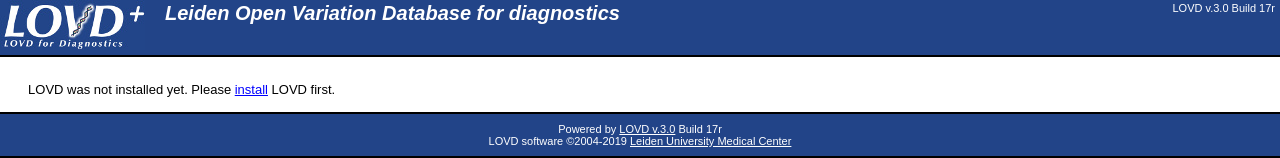
\includegraphics[width=\linewidth]{c02s02_screenshot_not_installed_plus.png}}%
  \caption{%
    When pointing your browser to the LOVD\textsuperscript{+} location, it will tell you it's not installed yet.
    Click the link to start the install process.}
  \end{shaded}
\end{figure}

\noindent
LOVD\textsuperscript{+} will first check a few requirements.
Both the PHP and MySQL versions will be checked, to make sure your LOVD\textsuperscript{+}
 will function properly on your webserver environment.
Also some settings of the web server, PHP and MySQL will be checked.
Finally, LOVD\textsuperscript{+} will check if your config file has been hidden.
If all looks well, LOVD\textsuperscript{+} will tell you all requirements are OK
 and you're ready to start installing LOVD\textsuperscript{+}.
\vskip \baselineskip

Installing LOVD\textsuperscript{+} consists of only 4 simple steps and will take only a couple of minutes, or less.

\begin{figure}[ht]
  \begin{shaded}
  \frame{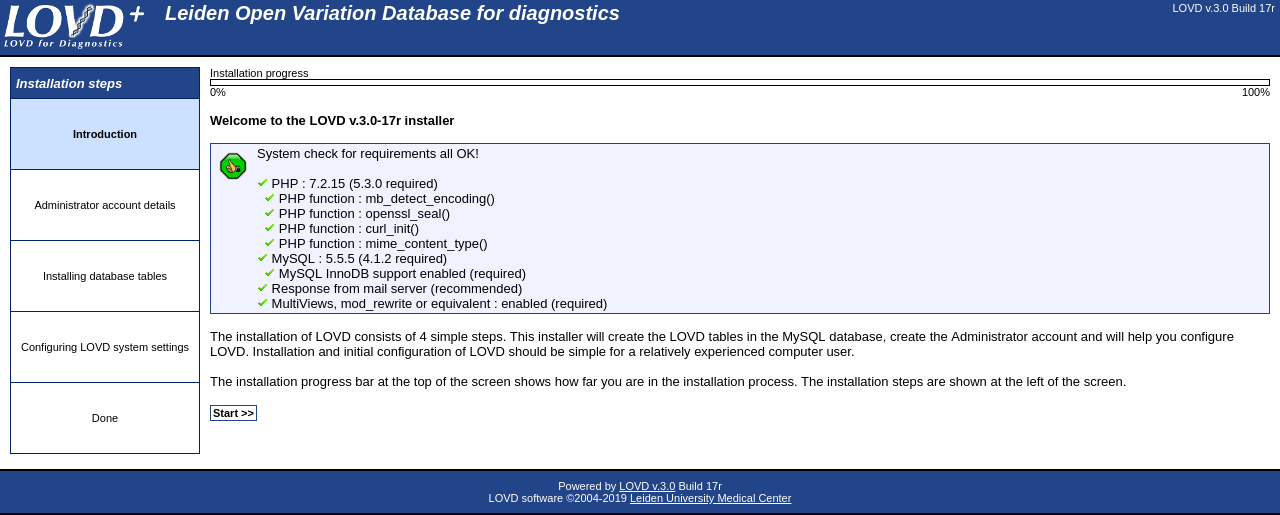
\includegraphics[width=\linewidth]{c02s02_screenshot_installer_01_plus.png}}%
  \caption{If all requirements are OK, you're ready to start installing LOVD\textsuperscript{+}.}
  \end{shaded}
\end{figure}



\subsection{Administrator account details}
Fill in the database administrator data to install LOVD\textsuperscript{+}.
The database administrator will be the first user registered with LOVD\textsuperscript{+}
 and has full access to all of LOVD\textsuperscript{+}'s functionalities.
The database administrator is the only user capable of creating manager accounts.
Managers can only create analyzer and read-only accounts.

\begin{figure}[ht]
  \begin{shaded}
  \frame{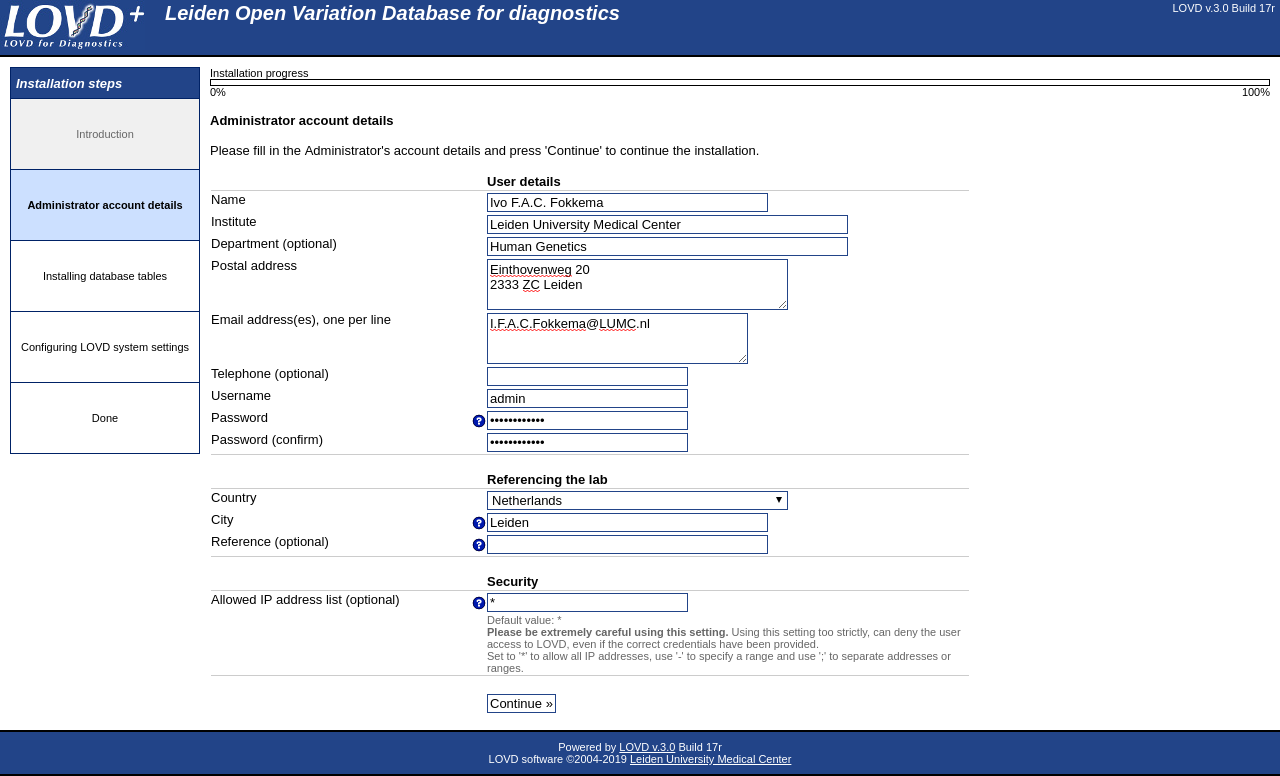
\includegraphics[width=\linewidth]{c02s02_screenshot_installer_02_plus.png}}%
  \caption{The database administrator registration form, with example data filled in.}
  \end{shaded}
\end{figure}

Most of the form is pretty straight forward, but I will highlight one field - ``Allowed IP address list''.
An IP address is an address a computer is known by on the network.
To help prevent others to try and guess the username/password combination,
 you can restrict access to the database administrator account to a number of IP addresses or ranges.
This also means you need to be very careful with this setting,
 as being too restrictive may lock you out of your account.
The default, unrestricted, value is *.

\begin{infotable}
The database administrator is the absolute owner of the LOVD\textsuperscript{+} installation.
Not only are they the only one that can uninstall LOVD\textsuperscript{+} from the database using the uninstaller,
 they will also be able to create, edit or delete all user accounts in the system and
 (depending on the settings) receive copies of emailed notifications.
\end{infotable}

\noindent
After completing the database administrator account details,
 click the ``Continue \guillemotright'' button at the bottom.
LOVD\textsuperscript{+} will apply a simple username and password quality check.
If LOVD\textsuperscript{+} tells you that the provided details are OK, click the ``Next \guillemotright'' button.



\subsection{Installing database tables}
The next step is to create and fill all necessary LOVD\textsuperscript{+} database tables.
LOVD\textsuperscript{+} will do this automatically,
 and you can watch the progress bar complete while the tables are created,
 the database administrator account created, the custom columns preconfigured,
 the standard columns enabled, and the standard analyses prepared.
This may take a while on non-optimal conditions, so please be patient.
When everything is done, a ``Next \guillemotright'' button appears - click it to continue.

\begin{figure}[ht]
  \begin{shaded}
  \frame{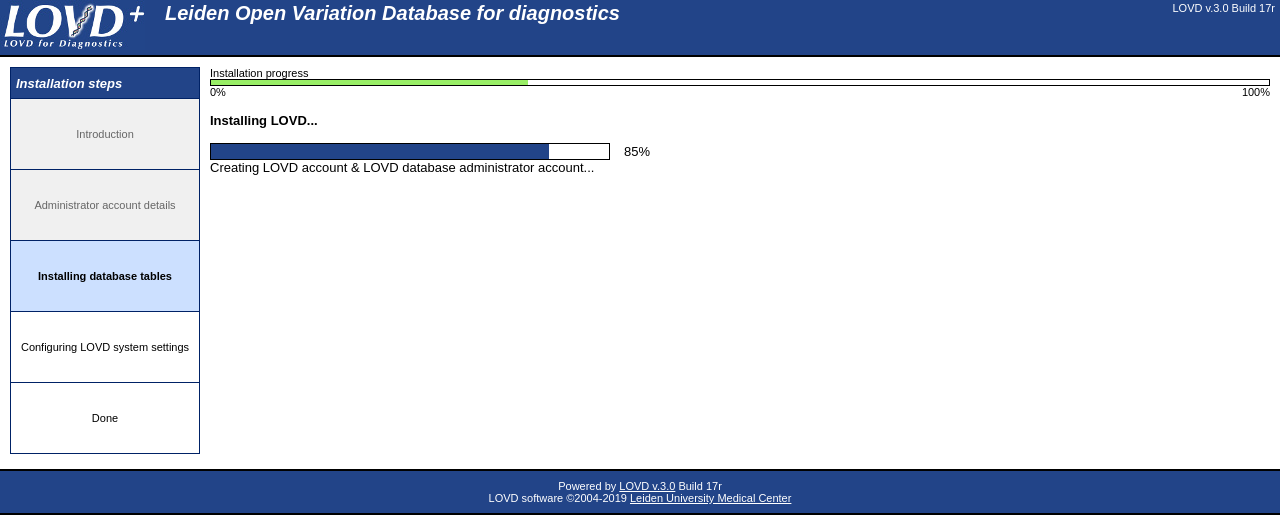
\includegraphics[width=\linewidth]{c02s02_screenshot_installer_03_plus.png}}%
  \caption{Watch the progress bar complete while LOVD\textsuperscript{+}
   informs you which part of the database table installation is currently in progress.}
  \end{shaded}
\end{figure}



\subsection{Configuring LOVD\textsuperscript{+} system settings}
The final form in the installation process is completing
 the initial configuration of the LOVD\textsuperscript{+} system settings.
These settings can be changed after installation at any time through the LOVD\textsuperscript{+} setup.

The only two settings that cannot be changed at a later time, are the install lock, which is checked by default,
 and the human build that the system will use to map your samples to.
Setting the uninstall lock will prevent uninstallation of LOVD\textsuperscript{+} by the database administrator.
The only way to remove this lock after installation is directly through the MySQL database backend.

\begin{figure}[ht]
  \begin{shaded}
  \frame{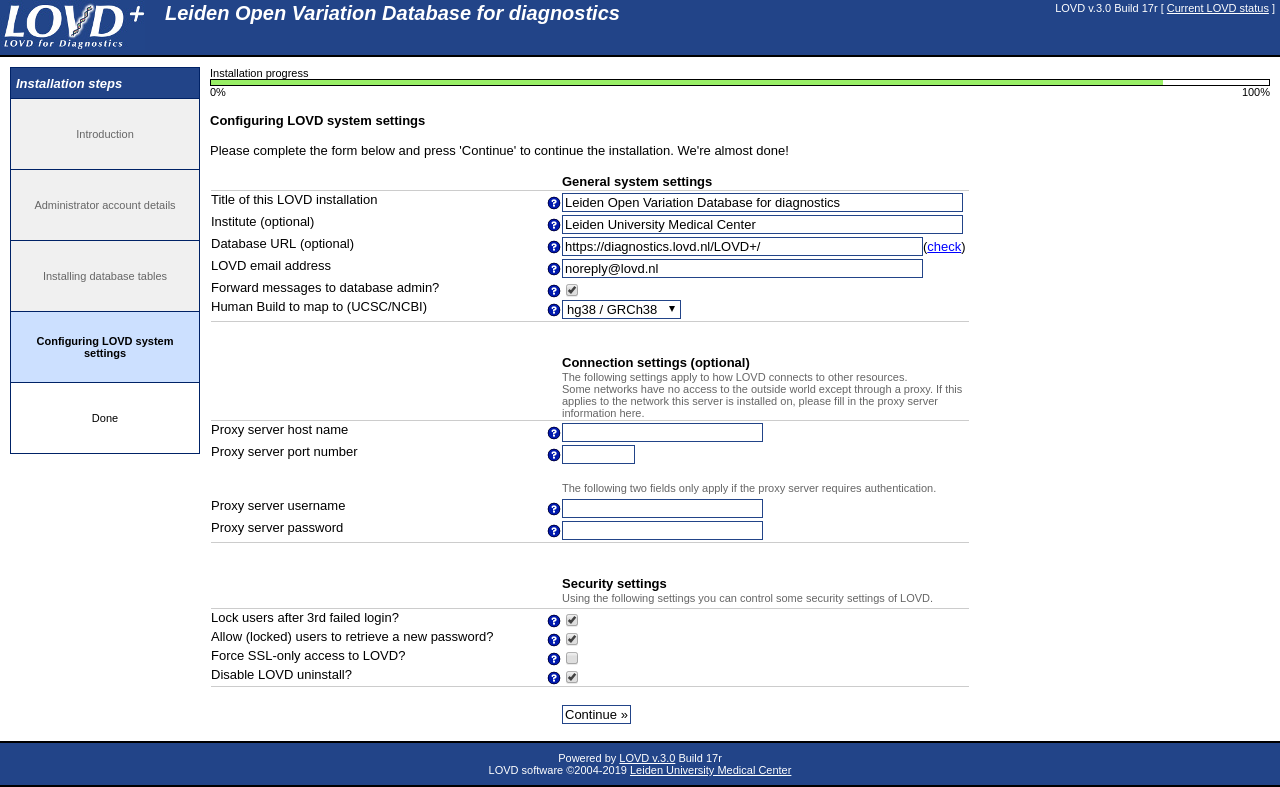
\includegraphics[width=\linewidth]{c02s02_screenshot_installer_04_plus.png}}%
  \caption{The system settings form, with example data filled in.}
  \end{shaded}
\end{figure}

\noindent
After filling in the form, click ``Continue \guillemotright''.
If everything was filled in correctly, LOVD\textsuperscript{+} will register
 the LOVD\textsuperscript{+} system settings.
Click ``Next \guillemotright'' to continue to the last step.
Almost done!



\subsection{Done}
When everything has been filled in and stored correctly, the installation is complete.
Now that you're done installing LOVD\textsuperscript{+}, click the ``Continue to Setup area \guillemotright'' button
 to be forwarded to the LOVD\textsuperscript{+} setup area.
From there, you can perform the most important actions for managers in LOVD\textsuperscript{+}, such as
 registering new user accounts, creating gene panels, managing custom columns and monitoring the import of data files.
The button to create a new gene panel will be highlighted, as a suggestion of your next step!










\chapter{Importing data}
\label{ch:importing_data}
LOVD\textsuperscript{+} can process one-sample or three-sample (trio) VCF files annotated with
 \href{http://www.ensembl.org/Homo_sapiens/Tools/VEP}{Ensembl VEP}, using RefSeq transcripts and preferably,
  with HGVS descriptions turned on.
Also tab-delimited files with VCF-style variant fields and the \href{http://www.LOVD.nl/3.0/docs}{LOVD import format}
 can be imported.
\vskip \baselineskip

As most users will begin with a VCF file, this chapter explains how LOVD\textsuperscript{+} can automatically process
 these files and how they can be automatically imported.
First, LOVD\textsuperscript{+} converts the VEP-annotated VCF files into tab-delimited files,
 with one line per the variant's annotation on a RefSeq transcript.
During this step, LOVD\textsuperscript{+} by default pre-filters your VCF files
 based on variant frequency or transcript annotation.
More on this below.
The tab-delimited files are subsequently converted into LOVD import files,
 while LOVD\textsuperscript{+} creates all the genes and transcripts in the system that are mentioned in the input file.
The resulting LOVD import file is then imported into LOVD\textsuperscript{+}.
Below all steps of the import process are explained, giving information how to automate these steps.





\section{Requirements}
\label{sec:import_requirements}
During the \hyperref[ssec:installing_pre-install_setup]{LOVD\textsuperscript{+} installation}
 you have already set path settings in your config.ini.php file.
The \texttt{data\_files} path is where you can store your VCF files to be processed,
 and the \texttt{data\_files\_archive} path is where the data files will be moved to after a successful import.
Please make sure these paths are correct, or LOVD\textsuperscript{+} can not function.
\vskip \baselineskip

LOVD\textsuperscript{+} does not include an annotation service and therefore relies on external annotation.
When using VCF files, LOVD\textsuperscript{+} is designed to work with
 \href{http://www.ensembl.org/Homo_sapiens/Tools/VEP}{Ensembl VEP}-annotated VCF files.
LOVD\textsuperscript{+} requires RefSeq annotation, so make sure you enable the option to use RefSeq transcripts.
Also, to speed up the conversion of the input data, configure VEP to include HGVS descriptions.
On the Ensembl VEP web interface, the HGVS option is found under ``Identifiers''.
When using the Ensembl VEP web interface, make sure you export your file in the ``VCF'' format.

Files from different annotation services like ANNOVAR might also work with minor configuration changes,
 if they can produce VCF files or tab-delimited files with one line per transcript.
However, we can not provide support on incorporating a different annotation service.
Contact \url{http://geneticreports.org/} to obtain support for LOVD\textsuperscript{+}.





\section{Processing VCF files}
\label{sec:import_vcf}
Make sure you have not more than one VCF file per individual, not separate VCF files.
You can have one or three samples in your VCF file.
When three samples are found, LOVD\textsuperscript{+} assumes you want to run trio-analysis
 and will take the three samples to be in the order Child, Father, Mother.
Each file name must end in \texttt{.vcf} to be recognized.
\vskip \baselineskip

Make sure your VCF files are stored in the correct folder (see ``\nameref{sec:import_requirements}'').
LOVD\textsuperscript{+} automatically searches for VCF files in this folder and converts them to tab-delimited files,
 when the \hyperref[sec:import_tsv]{conversion script} that processes tab-delimited files is run.
As such, to automatically process VCF files, see the section ``\nameref{sec:import_tsv}''.
\vskip \baselineskip

By default, variants with a frequency higher than 5\% in any population will be pre-filtered by the VCF file converter.
Also, variants without annotation on a gene are discarded,
 and only coding transcripts (\texttt{NM} and \texttt{XM}) are selected.
These settings can currently only be changed by editing the \texttt{\$\_CONFIG} header of the VCF file converter,
 where its settings are stored.
To turn off or edit the filtering in the VCF file converter, for now you'll need to edit the settings in the
 \texttt{vcf\_to\_tsv.php} file in the \texttt{scripts} directory.
See lines 76-82 for turning filters off (change \texttt{true} in \texttt{false}) and lines 84-123 for filter settings.
Note that editing the script directly will cause the changes to be overwritten when you update LOVD\textsuperscript{+},
 so in a later release the settings will be moved to a slightly better place.





\section{Processing tab-delimited files}
\label{sec:import_tsv}
Tab-delimited files, usually obtained from converted VEP-annotated VCF files,
 are converted to the LOVD import format by the \texttt{convert\_and\_merge\_data\_files.php} script.
This script takes a tab-delimited file, searches for an optional matching meta data file
 containing information about the individual, and merges them into a single LOVD import file.
The meta data file needs to be in the \href{http://www.LOVD.nl/3.0/docs/}{LOVD import format},
 containing the header and the \texttt{Diseases}, \texttt{Individuals},
 \texttt{Individuals\_To\_Diseases} and \texttt{Screenings} sections.
At least one Individual and one Screening need to be defined.
If no meta file exists, LOVD\textsuperscript{+} will create one with default information.
You can use such a default generated file as a template if you wish to provide meta data files.
Data file names must end in \texttt{.vep.data.lovd} to be recognized, although this can be configured. %% FIXME: How?
Meta data file names must end in \texttt{.meta.lovd} to be recognized (also configurable), %% Configurable where?
 and they must have the same prefix as the data file.
\vskip \baselineskip

Note that the first conversion will be slow, because while checking your file's annotation, LOVD\textsuperscript{+}
 will download information about genes and transcripts, and will create them in the database.
LOVD\textsuperscript{+} is not pre-populated with this information because it depends on your human build and
 annotation pipeline (such as the VEP version).
As gene and transcript information is loaded into LOVD\textsuperscript{+},
 your future file conversions will become faster.

\begin{warntable}
Note that, since the \texttt{convert\_and\_merge\_data\_files.php} script will create genes and transcripts in the
 database when it first encounters them, it is not recommended to run this script in parallel the first few runs.
Errors may occur when two parallel runs try to create the same gene or transcript.
If such error occurs, simply delete the \texttt{tmp} file that is created by the failed run, and run the script again.
\vskip \baselineskip

Also, when the conversion script just stops without warning,
 it's possible that it's using more memory than currently allowed.
You can edit the script to change the \texttt{memory\_limit} setting in the file's header.
\end{warntable}

\noindent
LOVD\textsuperscript{+} will search for tab-delimited files in the
 \texttt{data\_files} directory (see ``\nameref{sec:import_requirements}'').
Before searching for a tab-delimited file, LOVD\textsuperscript{+} will first locate VCF files that have not yet been
 converted yet, and convert one into a tab-delimited file.
As such, you do not need to run the VCF file converter separately.
Running the \texttt{convert\_and\_merge\_data\_files.php} script will suffice
 for obtaining LOVD import files from VCF files.
\vskip \baselineskip

To automate the file conversion on Linux servers,
 for any user with write access to the data directory create the cronjob as in figure \ref{fig:import_tsv_cronjob}.
To run it just once, open the \texttt{scripts} folder from your browser and run the
 \texttt{convert\_and\_merge\_data\_files.php} script.

\begin{figure}[ht]
  \begin{shaded}
\begin{verbatim}
*/15 * * * * php -f /path_to_LOVD+/scripts/convert_and_merge_data_files.php
\end{verbatim}
  \caption{%
    Example cronjob to facilitate automatic conversion of meta and data files into LOVD import files.
    Make sure the directory in which `php' resides, is in the PATH environment variable.
    Also, change ``\texttt{path\_to\_LOVD+}'' to the full path of your LOVD\textsuperscript{+} installation.
    Feel free to change the time settings, but note that running the conversion script in parallel
     may cause errors when the script is still creating genes and transcripts.
    The duration of a conversion run depends completely on the size of the file,
     and the number of genes and transcripts from the data file that are not yet imported into LOVD\textsuperscript{+}.
    The conversion of data files does not interfere with normal functionality of LOVD\textsuperscript{+},
     and as such can run 24 hours a day, also whenever LOVD\textsuperscript{+} is in use.}
    \label{fig:import_tsv_cronjob}
  \end{shaded}
\end{figure}





\section{Processing import files}
\label{sec:import_import}
Files converted into LOVD import files by LOVD\textsuperscript{+} are automatically scheduled to be imported.
If you're creating LOVD import files by yourself, you can schedule them through the
 ``\hyperref[sec:import_monitoring]{Schedule data files to be imported into LOVD\textsuperscript{+}}''
 feature in the Setup area.

Scheduled files can be imported by running the auto importer.
To facilitate automatic import of the scheduled import files on Linux servers,
 create the cronjob for a user of your choice as in figure~\ref{fig:import_import_cronjob}.
To run it just once, open the following URL, correctly inserting the address of your LOVD\textsuperscript{+}
 installation: \texttt{http://URL\_to\_LOVD+/import?autoupload\_scheduled\_file}.

\begin{infotable}
Although prefiltering your data on frequency is recommended, note that LOVD\textsuperscript{+}
 is able to import files up to 250MB.
However, your PHP settings may have additional limits, so if your file is rejected
 because it's too large but it's below 250MB, check your PHP settings.
LOVD\textsuperscript{+} can help you locate which setting needs to be adapted.
From the Setup menu button's dropdown menu, select ``Import data''.
Move your mouse over the small blue question mark near ``Select the file to import''.
\end{infotable}

\begin{figure}[ht]
  \begin{shaded}
  \small
\begin{verbatim}
*/15 0-5,19-23 * * * curl -L "http://URL_to_LOVD+/import?autoupload_scheduled_file"
\end{verbatim}
  \caption{%
    Example cronjob to facilitate automatic import of scheduled LOVD import files.
    Make sure the directory in which `curl' resides, is in the PATH environment variable.
    Using another downloader like `wget' is of course also possible, just make sure the output is sent to STDOUT and
     make sure the downloader doesn't time out (large files can take some time to import).
    Also, change ``\texttt{URL\_to\_LOVD+}'' to the full URL of your LOVD\textsuperscript{+} installation.
    Feel free to change the time settings, but note that since the import of large data files does slow down normal
     functionality of LOVD+, it is recommended to run the import only outside of working hours.}
    \label{fig:import_import_cronjob}
  \end{shaded}
\end{figure}
\clearpage % To prevent a very, very empty page a few pages further.





\section{Monitoring the progress and problem solving}
\label{sec:import_monitoring}
You can monitor the progress of your file conversion and your imports through LOVD\textsuperscript{+}.
From the setup area, click ``Schedule data files to be imported'',
 or from the setup menu tab drop down menu, select ``Schedule data for import''.
Although LOVD\textsuperscript{+} automatically schedules files for import after conversion, this screen can also be
 used to manage your imports, like prioritize them, and to troubleshoot file conversions and file imports.
See figure \ref{fig:c03s05_screenshot_import_scheduler_plus}
 for an overview of this page and all possible statuses you can find there.

\begin{figure}[ht]
  \begin{shaded}
    \frame{
      \begin{tikzpicture}
        \node[anchor=south west,inner sep=0] (image) at (0,0) {
          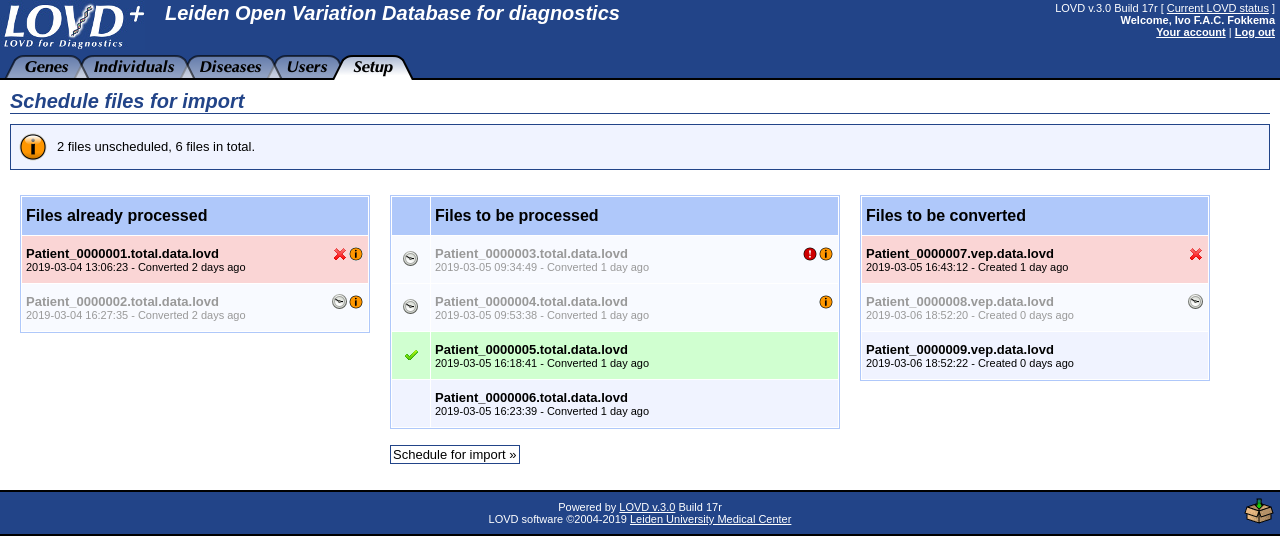
\includegraphics[width=\linewidth]{c03s05_screenshot_import_scheduler_plus.png}
        };
        \begin{scope}[x={(image.south east)},y={(image.north west)}]
          \tikzstyle{every node}=[circle,fill=\pointercolor,scale=0.6];
          \draw [red,thick,rounded corners] (0.668,0.280) rectangle (0.949,0.646);
          \node at (0.930,0.255) {\textbf{1}};
          \node at (0.880,0.517) {\textbf{4}};
          \node at (0.880,0.427) {\textbf{3}};
          \node at (0.880,0.337) {\textbf{2}};
          \draw [red,thick,rounded corners] (0.301,0.190) rectangle (0.660,0.646);
          \node at (0.640,0.165) {\textbf{5}};
          \node at (0.570,0.247) {\textbf{6}};
          \node at (0.570,0.337) {\textbf{7}};
          \node at (0.570,0.427) {\textbf{8}};
          \node at (0.570,0.517) {\textbf{9}};
          \draw [red,thick,rounded corners] (0.012,0.370) rectangle (0.293,0.646);
          \node at (0.270,0.337) {\textbf{10}};
          \node at (0.230,0.427) {\textbf{11}};
          \node at (0.230,0.517) {\textbf{12}};
          % \drawgrid
        \end{scope}
      \end{tikzpicture}}
    \caption{From this screen, you can manage your imports and troubleshoot any conversion or file import errors.}
    \label{fig:c03s05_screenshot_import_scheduler_plus}
  \end{shaded}
\end{figure}

\noindent
The scheduling screen shows all your data files that have not been imported yet, in three different columns.
The `flow' in which the files move is from the right to the left.
The far right table \circled{1} shows the VEP data files that have been created from VEP annotated VCF files.
New VEP data files, not yet converted to LOVD data files, show with a blue background \circled{2}.
When a file is picked up for conversion, it turns grey and shows a clock icon \circled{3}.
If a file failed to be converted due to annotation errors, it shows up as red \circled{4}.
Moving your mouse over the red cross shows you the error messages that occured.
They can also be seen in the \texttt{.error} file that will be created on disk.
\textbf{Note that by default, LOVD\textsuperscript{+} allows for 50 annotation errors during VEP file conversion.}
See \hyperref[sec:import_settings]{the next section} for how to change these settings.
When the conversion of a file fails, LOVD\textsuperscript{+} will not automatically try again,
 to make sure the conversion queue doesn't get stuck on this file.
If you want LOVD\textsuperscript{+} to try again,
 remove the sample's \texttt{.total.data.tmp} file from the data directory.
\vskip \baselineskip

Files successfully converted into LOVD data files show up in the middle column \circled{5}.
Unscheduled files are shown with a blue background \circled{6}.
Clicking them will mark them in green \circled{7}, after which
 they can be scheduled by clicking the ``Schedule for import'' button below the table.
Note however, that LOVD\textsuperscript{+} automatically schedules files for import.
Files scheduled for import are colored grey \circled{8},
 show a clock icon on their left, and show an information icon on their right.
Moving your mouse over the information icon shows you who has scheduled this file, and when.
Clicking the file shows a menu that allows you to prioritize the file or to unschedule it.
Prioritizing a file shows it at the top of the list \circled{9}, with a red exclamation mark next to it.
LOVD\textsuperscript{+} comes with three levels of priority; ``Default'', ``Medium priority'', ``High priority''.
This allows you to precisely mark the order in which files should be imported, in case you have many files to import.
\vskip \baselineskip

Files currently importing or where the import failed, are shown on the far left \circled{10}.
Currently importing files are shown in grey \circled{11} and show an clock icon as well as an information icon.
Moving your mouse over the information icon shows you who has scheduled this file, and when.
Moving your mouse over the clock icon shows you when the import has started.
In case the import fails, files are shown in red \circled{12} and show a red cross.
Moving your mouse over the red cross shows you the errors that were encountered during the import.
These errors are also shown in the output of the import script.
Clicking on a file in this list will show a menu that allows you to unschedule or to reschedule a file.
Rescheduling a previously failed file will clear the errors and will schedule the file to be imported again.
Unscheduling a file will simply put it back in the previous list \circled{5}.





\section{Adapting settings for file conversion}
\label{sec:import_settings}
Besides the VCF file converter's settings that currently still have to be changed \hyperref[sec:import_vcf]{in the
 script's header itself}, the settings for the VEP data file conversion into LOVD data files, can be controlled by
% FIXME: Add own chapter on this.
 editing the \emph{adapter library}.
The adapter library is a file meant to override default LOVD\textsuperscript{+} settings and features, by providing
 alternative configuration or functions performing certain tasks in LOVD\textsuperscript{+}.
As these settings and features are stored in a new file, they still safely allow updating
 LOVD\textsuperscript{+} to newer versions without the chance of overwriting your settings.
In the future, more LOVD\textsuperscript{+} settings and features may be moved into the adapters.
\vskip \baselineskip

To adapt LOVD\textsuperscript{+} settings and features through the adapter,
 you can either create your own adapter files containing your changes, or you can edit the default adapter files.



\subsection{Using your own adapter files}
\label{ssec:adapters_using_your_own}
Using your own adapter files to adapt LOVD\textsuperscript{+} settings and features
 is the best way to change settings or features, but it is not the easiest way.
It is the best way because it makes LOVD\textsuperscript{+} easy to update;
 changes to LOVD\textsuperscript{+} will never overwrite your changes as they are in separate files.
However, it requires you to create a new file and edit the configuration
 file to make sure LOVD\textsuperscript{+} knows it has to use your file.
These are the steps to create your own adapter library, containing settings for LOVD\textsuperscript{+}:

\begin{description}
  \item[Think of a name for your LOVD\textsuperscript{+} instance] \hfill \\
    Your adapter files need to be named after your \emph{instance name}.
    Think of an name for your LOVD\textsuperscript{+} instance, for example your institute's name.
    Instance names in use are for example \texttt{leiden} or \texttt{MGHA}.
    In this manual's examples, we'll use \texttt{example} as the instance name of your choice.
  \item[Create an empty file named \texttt{adapter.lib.EXAMPLE.php}] \hfill \\
    All relevant files are in the \texttt{scripts/adapters/} directory.
    Create a new file there with the name \texttt{adapter.lib.EXAMPLE.php},
     replacing \texttt{EXAMPLE} with your chosen instance name (make sure your instance name is in \emph{all capitals}).
  \clearpage % To prevent a very, very empty page a few pages further.
  \item[Edit your new file] \hfill \\
    Simply edit your new \texttt{adapter.lib.EXAMPLE.php} file and change the settings you want to change.
    To keep it simple, define and set only the settings you want to change.
    Since these adapter files are PHP files that can contain functions as well as simple settings,
     they need to be in PHP format.
    See figure \ref{fig:adapters_new_file} for an example.
  \item[Tell LOVD\textsuperscript{+} to use your new file] \hfill \\
    Finally, tell LOVD\textsuperscript{+} to use your new file.
    Do so by editing the \texttt{config.ini.php} file in the LOVD\textsuperscript{+} directory.
    Find the \texttt{[instance]} section and fill in the \texttt{name} setting.
    See figure \ref{fig:adapters_instance_name} for an example.
\end{description}

\begin{figure}[ht]
  \begin{shaded}
    \small
    \begin{verbatim}
<?php
// Allow conversions to run into more annotation errors than the default 50.
$_INSTANCE_CONFIG['conversion']['annotation_error_max_allowed'] = 500;

// We'll make our own meta files, don't let LOVD+ make any.
$_INSTANCE_CONFIG['conversion']['create_meta_file_if_missing'] = false;

// Speeds up the conversion.
$_INSTANCE_CONFIG['conversion']['check_indel_description'] = false;
?>
\end{verbatim}
  \caption{%
    An example of an adapter library file, changing only a few settings from the defaults.
    Lines starting with two slashes are comments.}
    \label{fig:adapters_new_file}
  \end{shaded}
\end{figure}

\begin{figure}[ht]
  \begin{shaded}
    \small
    \begin{verbatim}
[instance]

# The name of this instance, used to activate site specific features.
name = example
\end{verbatim}
  \caption{%
    The \texttt{[instance]} section of the \texttt{config.ini.php} file, with the instance name configured.
    In this example the instance name is \texttt{example}.}
    \label{fig:adapters_instance_name}
  \end{shaded}
\end{figure}



\subsection{Editing the default adapter}
\label{ssec:adapters_editing_the_default}
By far the easiest way however to change the default settings, is to edit the default adapter.
It allows you to quickly check the effect of changes to the default settings,
 and you don't need to create any new files for this.
However, this means that when you update LOVD\textsuperscript{+}, you'll have to re-apply your changes to the settings.
If you prefer this method, simply navigate to the \texttt{scripts/adapters}
 folder and edit the \texttt{adapter.lib.DEFAULT.php} file.
Once you save the changes to the file, LOVD\textsuperscript{+} will use the new settings.
\clearpage % To prevent a very, very empty page a few pages further.



\subsection{Which settings can be changed}
\label{ssec:adapters_which_settings}
The default adapter has a lot of settings and features in them that you can change.
This is not the full list, but these are the changes that are relevant for the data file conversions.

\begin{description}
  \item[conversion] \hfill \\
    This is a container containing all the file conversion related settings.
  \begin{description}
    \item[annotation\_error\_drops\_line] \hfill \\
      Should we discard the variant's mapping on this transcript completely when we run into annotation errors?
      Annotation errors are, for instance, not being able to generate a DNA description or
       not being able to generate a protein change prediction.\\
      Valid values: \texttt{false}, \texttt{true}.\\
      Default value: \texttt{false}.
    \item[annotation\_error\_exits] \hfill \\
      Set whether to halt on the first annotation error.\\
      Valid values: \texttt{false}, \texttt{true}.\\
      Default value: \texttt{false}.
    \item[annotation\_error\_max\_allowed] \hfill \\
      Set here the maximum number of errors with transcript mappings before the script halts anyway.
      How many annotation errors might occur, depends on your annotation pipeline.
      In small files up to $\sim$25.000 variants, annotation errors might not occur at all.
      If you're getting a lot of annotation errors, please verify if your
       LOVD\textsuperscript{+} is using the same genome build as the file you're trying to convert.\\
      Valid values: whole numbers above zero.\\
      Default value: \texttt{50}.
    \item[create\_genes\_and\_transcripts] \hfill \\
      When LOVD\textsuperscript{+} encounters a gene or transcript it hasn't seen before, it can automatically create
       these genes and transcripts in the database.
      This process can be slow at first, but prevent annotation errors to occur
       when your database doesn't contain all genes and transcripts yet.
      Since by default, LOVD\textsuperscript{+} doesn't come with all gene and transcript information loaded,
       without this setting you won't be able to import any mappings onto genes and transcripts at first.\\
      Valid values: \texttt{false}, \texttt{true}.\\
      Default value: \texttt{true}.
    \item[create\_meta\_file\_if\_missing] \hfill \\
      LOVD\textsuperscript{+} requires a meta data file with each sample,
       defining information line gender, phenotype, etc.
      However, since the creation of this file (in the LOVD import format) is not trivial,
       LOVD\textsuperscript{+} can just create a meta file with default settings if it's missing.\\
      Valid values: \texttt{false}, \texttt{true}.\\
      Default value: \texttt{true}.
    \item[check\_indel\_description] \hfill \\
      Ensembl VEP doesn't do a very good job at predicting the DNA change
       on the transcript level for deletions or insertions.
      Should LOVD\textsuperscript{+} check all indel descriptions using Mutalyzer?
      This will slow down the data file conversion a bit,
       but will provide higher quality DNA descriptions on the transcript level.\\
      Valid values: \texttt{false}, \texttt{true}.\\
      Default value: \texttt{true}.
    \clearpage % To prevent a very, very empty next page.
    \item[enforce\_hgnc\_gene] \hfill \\
      When LOVD\textsuperscript{+} encounters a new gene symbol in the VEP data file,
       should LOVD\textsuperscript{+} check if this is a correct gene symbol in the HGNC database?
      This setting makes only sense when you have \texttt{use\_hgnc} set to \texttt{true}.\\
      Valid values: \texttt{false}, \texttt{true}.\\
      Default value: \texttt{true}.
    \item[use\_hgnc] \hfill \\
      Use the HGNC to collect gene information when LOVD\textsuperscript{+} finds a new gene symbol?
      This setting makes only sense when you have \texttt{create\_genes\_and\_transcripts} set to \texttt{true}.\\
      Valid values: \texttt{false}, \texttt{true}.\\
      Default value: \texttt{true}.
    \item[verbosity\_cron] \hfill \\
      When LOVD\textsuperscript{+} recognizes that the conversion script is automated through cron,
       how much information should it output?
      This is to prevent detailed output from showing up when the process is not directly monitored, anyway.\\
      Valid values: \texttt{0} (no output), \texttt{3}, \texttt{5}, \texttt{7}, \texttt{9} (full debugging output).\\
      Default value: \texttt{5}.
    \item[verbosity\_other] \hfill \\
      In all other cases, how much information should the conversion script output?\\
      Valid values: \texttt{0} (no output), \texttt{3}, \texttt{5}, \texttt{7}, \texttt{9} (full debugging output).\\
      Default value: \texttt{7}.
  \end{description}
\end{description}










\chapter{Running analyses}
\label{chap:running_analyses}
\section{Listing the imported samples}
\label{sec:running_analyses_data_listing}

Once samples have been imported, they are shown in the Individuals listing,
 available from the ``Individuals'' menu tab.
See figure \ref{fig:individuals_listing_plus}.

\begin{figure}[ht]
  \begin{shaded}
    \frame{
      \begin{tikzpicture}
        \node[anchor=south west,inner sep=0] (image) at (0,0) {
          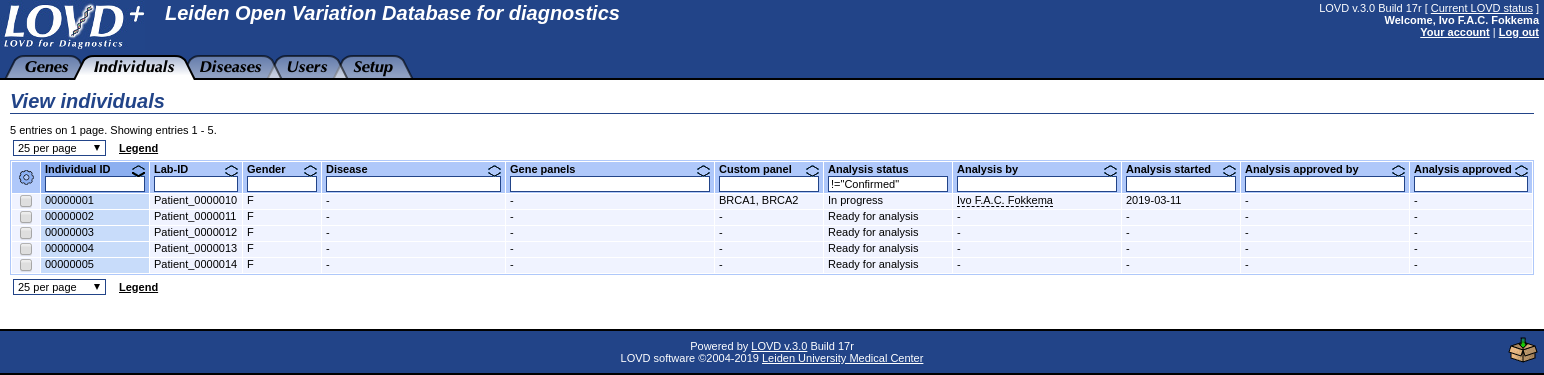
\includegraphics[width=\linewidth]{individuals_listing_plus.png}
        };
        \begin{scope}[x={(image.south east)},y={(image.north west)}]
          \tikzstyle{every node}=[circle,fill=\pointercolor,scale=0.6];
          \node at (0.600,0.595) {\textbf{1}};
          \node at (0.190,0.630) {\textbf{2}};
          \draw [red,thick,rounded corners] (0.096,0.255) rectangle (0.210,0.585);
          \node at (0.300,0.595) {\textbf{3}};
          \node at (0.430,0.630) {\textbf{4}};
          \draw [red,thick,rounded corners] (0.326,0.255) rectangle (0.535,0.585);
          \node at (0.790,0.630) {\textbf{5}};
          \draw [red,thick,rounded corners] (0.615,0.255) rectangle (0.994,0.585);
          % \drawgrid
        \end{scope}
      \end{tikzpicture}}
    \caption{The list of samples imported into LOVD\textsuperscript{+}.}
    \label{fig:individuals_listing_plus}
  \end{shaded}
\end{figure}

\noindent
Note, that the list of individuals, by default, does not show individuals that are marked as ``Confirmed''
 (i.e. analysis completed).
You can disable this filter, or change the filter,
 by removing the value in the ``Analysis status'' filter field \circled{1} and pressing the enter key.
\vskip \baselineskip

The left of the listing shows custom fields available for Individuals \circled{2}.
The ``Lab-ID'' column shows the sample's file name or configured Lab ID from the sample's prepared meta data file.
The ``Gender'' field can also be provided from a prepared meta data file,
 or can be filled in by editing the Individual entry after import has completed.
Also the ``Disease'' can be pre-configured using a prepared meta data file or added later.
Diseases need to be configured in the system (``Diseases'' menu tab) and can be assigned to gene panels
 (``Genes'' menu tab) in order to easily assign gene panels.
Gene panels \circled{4} are used to quickly focus variant filtering on genes already known
 to be associated with the condition of the individual analyzed.
LOVD\textsuperscript{+} allows you also to choose a `custom panel', in addition to a normal gene panel,
 to focus on genes you wish to select for this sample only.
A custom panel can also be used to temporarily add a few genes to an existing gene panel.
Gene panels linked to individuals are listed in the ``Gene panels'' field.
The ``Custom panel'' field mentions the separate gene list configured for this individual.
The last few columns in the listing \circled{5} show information on who ran the first analysis on this individual and
 the date the analysis started, as well as information on when and by whom the analysis was approved.
\vskip \baselineskip

Although you can start off using custom panels; if you haven't created any gene panels yet,
 you probably want to do so first.
Click the ``Genes'' menu tab to see available gene panels.
To create one, move your mouse over the ``Genes'' menu tab, and click ``Create a new gene panel'' in the drop down menu.
\vskip \baselineskip

Click an individual to see your options.





\section{Overview of the analysis page}
\label{sec:running_analyses_page_overview}

The individual's analysis page allows you to check the individual's sequencing runs, analyze and filter these for
 causative variants, label and curate variants of interest, download the analysis results, and close the analysis.
See figure \ref{fig:individuals_analysis_page_plus} for the default analysis page.

\begin{figure}[ht]
  \begin{shaded}
    \frame{
      \begin{tikzpicture}
        \node[anchor=south west,inner sep=0] (image) at (0,0) {
          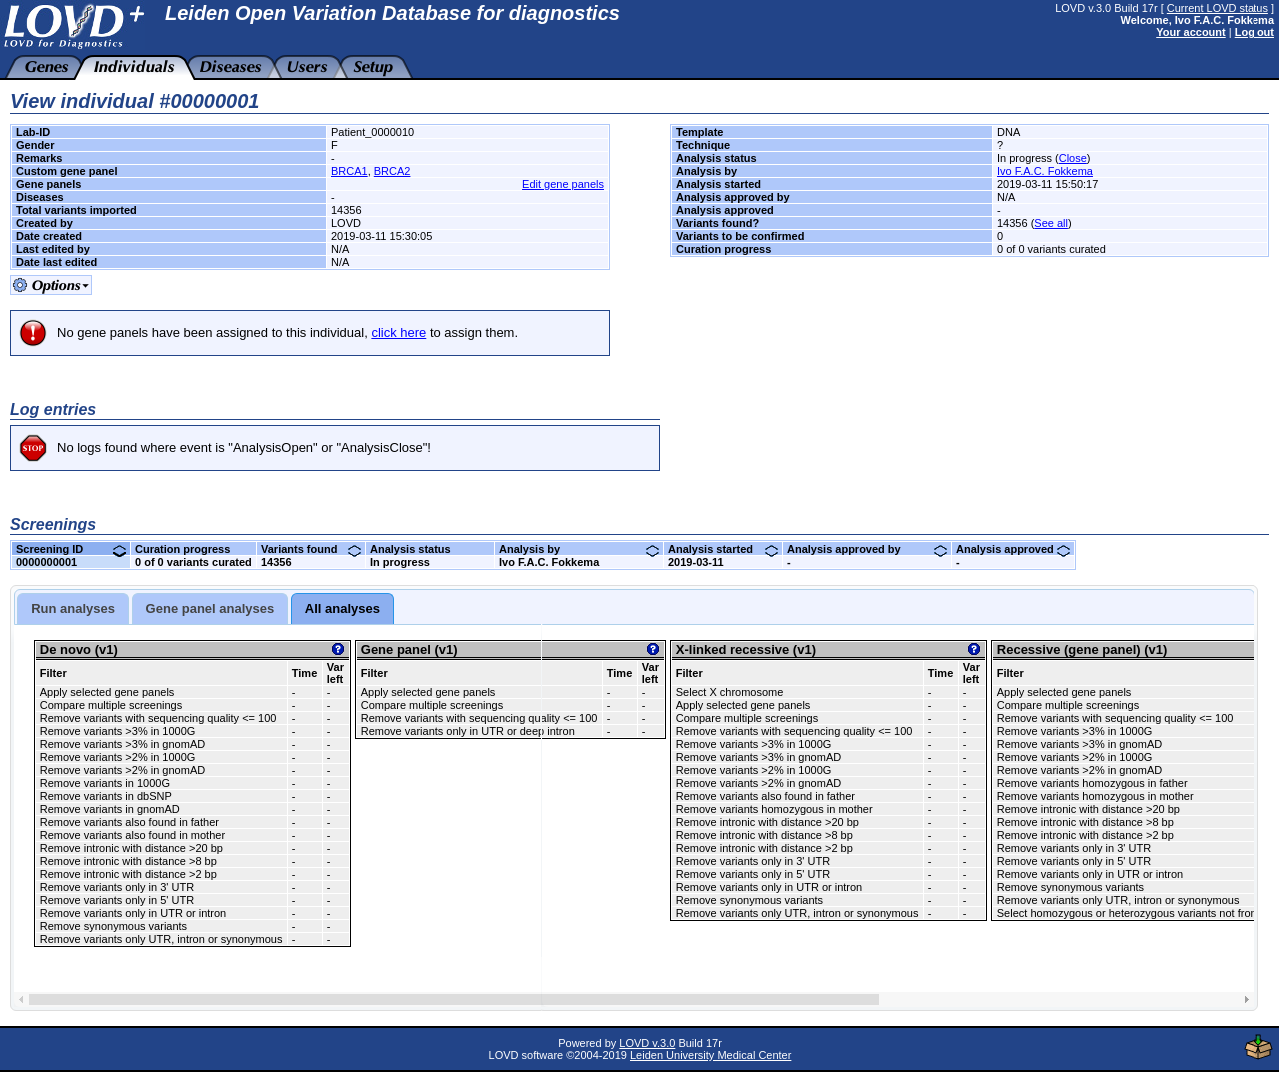
\includegraphics[width=\linewidth]{individuals_analysis_page_plus.png}
        };
        \begin{scope}[x={(image.south east)},y={(image.north west)}]
          \tikzstyle{nofill}=[draw,circle,red,thick,scale=0.8];
          \tikzstyle{yesfill}=[circle,fill=\pointercolor,scale=0.6];
          \node at (0.390,0.825) [yesfill] {\textbf{1}};
          \node at (0.450,0.582) [yesfill] {\textbf{2}};
          \node at (0.860,0.482) [yesfill] {\textbf{3}};

          \node at (0.890,0.865) [yesfill] {\textbf{4}};
          \draw [red,thick,rounded corners] (0.773,0.845) rectangle (0.880,0.886);

          \node at (0.890,0.792) [yesfill] {\textbf{5}};
          \draw [red,thick,rounded corners] (0.773,0.782) rectangle (0.880,0.801);

          \node at (0.330,0.435) [yesfill] {\textbf{6}};
          \node at (0.710,0.085) [yesfill] {\textbf{7}};

          \node (n1) at (0.5105,0.3945) [nofill] {};
          \node (n2) at (0.450,0.260) [yesfill] {\textbf{8}};
          \draw [red,thick] (n1) -- (n2);
          % \drawgrid
        \end{scope}
      \end{tikzpicture}}
    \caption{The default analysis page for a new sample that has not been analyzed yet.}
    \label{fig:individuals_analysis_page_plus}
  \end{shaded}
\end{figure}



\subsection{Data on the individual and the sequencing analysis}
On the top left of the page, the individual's basic information is shown.
You can configure the individual's gene panels here, by clicking the ``Edit gene panels'' link \circled{1}
 or the link in the message just below the individual's basic information.
You can also paste a list of gene symbols in the ``Custom gene panel'' field on that page.
Before you can use any gene panel filters, you will need to assign a gene panel here.
\vskip \baselineskip

Directly below the individual information pane, the ``Log entries'' section shows
 log entries related to this individual's analyses \circled{2}.
When analyses are closed or reopened, the log entries will be listed in this section.
This provides a history for the current status of the analysis.
\vskip \baselineskip

Under ``Screenings'', the sequencing runs performed on this individual are listed \circled{3}.
The selected sequencing run is printed in bold.
If a sequencing run has been selected, the top right of the screen
 displays the selected screening's statistics \circled{4}.
Shown are the defaults if no data has been provided through a prepared meta data file.
Having your sequencing pipeline create a meta data file allows you to, for instance, display detailed quality control.
The link to close an analysis is located right below the sequencing run statistics.
Closing an analysis will stop you from running any further analyses or make other changes.
There are various levels of closing an analysis.
By default they are `Closed', `Awaiting confirmation', and `Confirmed'.
Finally, the display includes the total number of variants imported \circled{5},
 as well as the link to display them all (unfiltered view).
\vskip \baselineskip



\subsection{Available analyses}
The list of available analyses is shown below the list of sequencing runs \circled{6}.
The ``Run analyses'' tab shows analyses that you have run before, the ``Gene panel analyses''
 tab shows analyses that are selected to be especially relevant for the gene panel(s) selected for this individual,
 and the ``All analyses'' tab shows all analyses available in this LOVD\textsuperscript{+} installation.
The ``Gene panel analyses'' tab is used in situations where many different gene panels have been defined.
Note that, depending on your screen size, you may need to scroll horizontally to see all analyses.
If so, a scroll bar will appear below the analysis list \circled{7}.
\vskip \baselineskip

Each analysis consists of a series of filter steps that are run one after the other from top to bottom,
 filtering the variants, to zoom in on candidate variants that may cause the individual's health problems.
The broadest filters are on top, more specific filters are at the bottom.
When the results of the analysis provide a too narrow view (e.g. no remaining variants),
 filters can be skipped (removed) from an analysis run.
In a later release, analyses can be customized for your specific needs through the Setup area.
Each analysis has a description that will show when moving your mouse over the questionmark icon \circled{8}.
Also each filter has a description that will be shown when you hover the filter name.





\section{Running analyses}
\label{sec:running_analyses_running}
To run an analysis, move your mouse over one of the grey analysis boxes (you will see the text
 ``Click to run this analysis'' appear at the bottom of the analysis), and click anywhere on the box.
A new dialog pops up, requesting configuration of the analysis.
What the dialog shows, depends on the active filters.
If the ``Apply selected gene panels'' filter is active,
 the configuration dialog will ask you to select which gene panel(s) will be active this analysis run.
If the ``Compare multiple screenings'' filter is active, the configuration dialog will show a form that allows
 you to select only variants that are also, or are not, present in other screenings.
If you have imported other family members as separate individuals, this feature can be used to only select variants not
 present in parents or also present in an affected family member, for instance.
This filter also allows you to select for a certain zygosity, allowing you to run analyses in complex families.

\begin{infotable}
Please note that although this filter will allow you to do basic trio analysis as well, it is far easier
 for you to use the standard LOVD\textsuperscript{+} procedure for this, by importing the trio as one sample.
See section ``\nameref{sec:import_vcf}'' for more information.
\end{infotable}

\noindent
You can usually leave the configuration dialog to its defaults.
Click ``Submit'' to run the analysis.
Usually, analyses run and complete within one or a few seconds.
This mainly depends on the number of variants you imported (see section ``\nameref{sec:import_vcf}''
 about filtering of the VCF file) and on whether or not you have selected a gene panel.
The gene panel filter runs very fast and greatly reduces the number of variants to process further.
Figure \ref{fig:individuals_analysis_run_plus} shows an example of one run analysis with its results.

\begin{figure}[ht]
  \begin{shaded}
    \frame{
      \begin{tikzpicture}
        \node[anchor=south west,inner sep=0] (image) at (0,0) {
          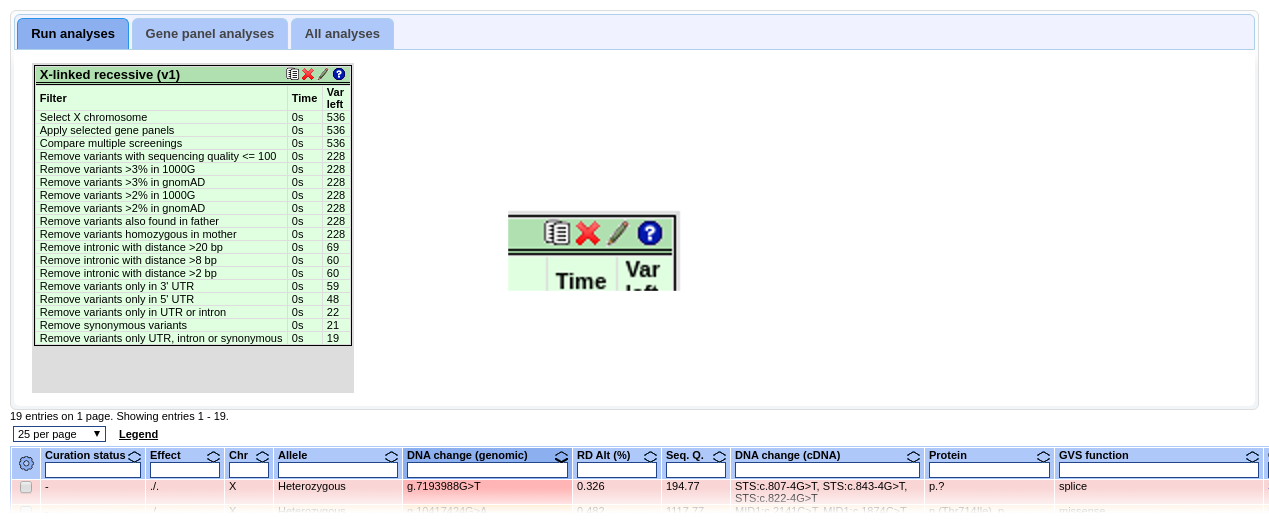
\includegraphics[width=\linewidth]{individuals_analysis_run_plus.png}
        };
        \begin{scope}[x={(image.south east)},y={(image.north west)}]
          \tikzstyle{nofill}=[draw,circle,red,thick,scale=1.1];
          \tikzstyle{yesfill}=[circle,fill=\pointercolor,scale=0.6];
          \node at (0.050,0.292) [yesfill] {\textbf{1}};
          \node at (0.270,0.155) [yesfill] {\textbf{2}};

          \draw [red,thick,rounded corners] (0.025,0.708) rectangle (0.150,0.765);
          \node at (0.160,0.765) [yesfill] {\textbf{3}};

          \draw [red,thick,rounded corners] (0.253,0.336) rectangle (0.277,0.792);
          \node at (0.290,0.420) [yesfill] {\textbf{4}};

          \draw [gray,thick] (0.280,0.875) -- (0.533,0.600);
          \draw [gray,thick] (0.280,0.775) -- (0.400,0.445);

          \node (n1) at (0.439,0.553) [nofill] {};
          \node (n2) at (0.434,0.350) [yesfill] {\textbf{5}};
          \draw [red,thick] (n1) -- (n2);

          \node (n3) at (0.463,0.553) [nofill] {};
          \node (n4) at (0.463,0.350) [yesfill] {\textbf{6}};
          \draw [red,thick] (n3) -- (n4);

          \node (n5) at (0.487,0.553) [nofill] {};
          \node (n6) at (0.492,0.350) [yesfill] {\textbf{7}};
          \draw [red,thick] (n5) -- (n6);

          % \drawgrid
        \end{scope}
      \end{tikzpicture}}
    \caption{An example of one run analysis with its results.
      Note the action buttons on the top right of the analysis box.}
    \label{fig:individuals_analysis_run_plus}
  \end{shaded}
\end{figure}

\noindent
An analysis that has been run, shows up as a green box.
The analysis that has currently been selected, has a grey band beneath it \circled{1}.
The analysis results of the currently selected analysis are displayed at the bottom of the screen \circled{2}.
Results are color coded based on the predicted effect on the protein.
Variants giving a frame shift, a premature translation termination (nonsense) codon and variants
 in the splice acceptor or donor sites are marked red; in-frame deletions or insertions and amino acid substitution
 (missense) variants in the coding region are orange;
 silent (synonymous) variants and variants in the 5'/3' UTR (untranslated region) or intron are marked green;
 other variants or variants with more than one effect due to their presence on multiple transcripts are marked blue.
\vskip \baselineskip

Once an analysis has been run, its table shows useful statistics.
Filters that have settings, such as the gene panel filter,
 show the settings that were active when the analysis was run \circled{3} (in this example, no settings have been set).
The rightmost column shows, per filter, the number of variants remaining after filtering completed \circled{4}.
\vskip \baselineskip

On the top right hand side of an analysis run table, some controls are provided, enlarged on the screenshot above.
The controls allow you to:
\begin{itemize}
  \setlength\itemsep{0em}
  \item \circled{5} Duplicate an analysis run to repeat it using, for instance, a different gene panel;
  \item \circled{6} Remove an analysis run if you wish to discard its results;
  \item \circled{7} Edit an analysis run if you wish re-run it disabling one or more of its filters.
\end{itemize}





\end{document}%%%%%%%%%%%%%%%%%%%%%%%%%%%%%%%%%%%%%%%%%%%%%%%%%%%%%%%%%%%%%%%%%%%%%%%%%%%%%%%%%%%%%%%%%%%%%%%%%%%%%%%%%%
%%%%%%%%%%%%%%%%%%%%%%%%%%%%%%%%%%%%%%%%%% NEW MAXIMUM LINE LENGTH (120 char) %%%%%%%%%%%%%%%%%%%%%%%%%%%%%%%%%%%%%%%%%%
